% https://tex.stackexchange.com/questions/123106/detect-aspect-ratio-in-beamer?noredirect=1&lq=1
\documentclass[aspectratio=169]{beamer}
%\documentclass[]{beamer}
%\usepackage{eulervm}
%\usetheme{metropolis} % Use metropolis theme
\usepackage[conference]{beamertheme_tumtalk} % headline and footline
\usepackage{beamercolorscheme_tum} % colorscheme
\usepackage{beamerfontthemestructurebold} % bold headings

\usepackage{appendixnumberbeamer}
\renewcommand\footnoterule{}


\usepackage[utf8]{inputenc}
\usepackage[T1]{fontenc}
\usepackage[autostyle, english = british]{csquotes}
\usepackage[british]{babel}
\usepackage{todonotes}
\usepackage[%
  backend=biber,
  doi=false,
  url=false,
  isbn=false,
  eprint=false,
  style=verbose,
  citestyle=verbose,
  hyperref=true,
  maxnames=99,
  minnames=1,
  maxbibnames=99,
  firstinits,
  uniquename=init]{biblatex}
%\DeclareFieldFormat[inproceedings, article]{pages}{}%
%\DeclareFieldFormat[inproceedings]{organization}{}%
  % ignore some field for citations
\DeclareSourcemap{
  \maps[datatype=bibtex, overwrite]{
    \map{
      \step[fieldset=edition, null]
      \step[fieldset=publisher, null]
      \step[fieldset=pages, null]
      \step[fieldset=organization, null]
    }
  }
}

\addbibresource{../bibliography.bib}

\let\oldfootnotesize\footnotesize
\renewcommand*{\footnotesize}{\oldfootnotesize\fontsize{6}{6}}

\usepackage{caption}
\usepackage{xpatch}
\usepackage{xcolor}
\usepackage{amsmath}
\usepackage{mathtools} % for \mathclap
\usepackage{nicefrac}
\usepackage{physics} % for derivatives
\usepackage{varioref}
\usepackage{siunitx}
\usepackage{hyperref}
\usepackage[noabbrev]{cleveref}
\newcommand{\creflastconjunction}{, and\nobreakspace} % use Oxford comma
\usepackage{todonotes}
\usepackage{multimedia}

\graphicspath{{../figures/}}
\let\boundary\undefined%

\usepackage{bm}


% Commands/Macros
% Names of methods or so
\newcommand{\muscl}{\textsc{muscl}-Hancock}
\newcommand{\dg}{\textsc{dg}}
\newcommand{\ader}{\textsc{ader}}
\newcommand{\aderdg}{\textsc{ader-dg}}
\newcommand{\amr}{\textsc{amr}}
\newcommand{\pde}{\textsc{pde}}
\newcommand{\cpp}{C\texttt{++}}
\newcommand{\tbb}{\textsc{tbb}}
\newcommand{\mpi}{\textsc{mpi}}

\newcommand{\softwareName}[1]{\textit{#1}}
\newcommand{\exahype}{\softwareName{ExaHyPE}}
\newcommand{\peano}{\softwareName{Peano}}
\newcommand{\className}[1]{\texttt{#1}}
\newcommand{\funName}[1]{\textsf{#1}}
\newcommand{\fileName}[1]{\textbf{#1}}
\newcommand{\varName}[1]{\enquote{#1}}



% Variables and other equation stuff
\newcommand{\Q}{\bm{Q}}
\newcommand{\gradQ}{\gradient{\Q}}
\newcommand{\Qrho}{\rho}
\newcommand{\Qj}{\rho \bm{v}}
\newcommand{\Qv}{\bm{v}}
\newcommand{\QE}{\rho E}
\newcommand{\QZZ}{Z} % TODO: Name?
\newcommand{\QZ}{\rho \QZZ}
\newcommand{\potT}{\theta}
\newcommand{\backgroundPotT}{\overline{\theta}}
\newcommand{\pertubationPotT}{\theta'}
\newcommand{\stressT}{\bm{\sigma}}
\newcommand{\pressure}{p}
\newcommand{\maxConvEigen}[1][]{
  \vert%
  \lambda_c^{\text{max}}
  \notblank{#1}{\left(#1\right)}{}
  \vert%
}
\newcommand{\maxViscEigen}[1][]{
  \vert%
  \lambda_v^{\text{max}}
  \notblank{#1}{\left(#1\right)}{}
  \vert%
}
\newcommand{\Riemann}{\operatorname{Riemann}}

% Domain
\newcommand{\domain}{\Omega}
\newcommand{\boundary}{\partial \domain}
\newcommand{\broken}{\domain}

% Cells
\newcommand{\cell}[1][]{C_{#1}}
\newcommand{\refCell}[1][]{\hat{C}_{#1}}
\newcommand{\cellb}{\partial{} \cell}
\newcommand{\refCellb}{\partial{} \refCell}

% Basis functions
\newcommand{\lagrange}[1][i]{\varphi_{#1}}
\newcommand{\lagrangeRef}[1][i]{\hat{\varphi}_{#1}}
\NewDocumentCommand{\sbasis}{ O{} O{} }{\phi^{#1}_{#2}}
\NewDocumentCommand{\sbasisRef}{ O{} O{} }{\hat{\phi}^{#1}_{#2}} %{\hat{\sbasis[#1][#2]}}
\NewDocumentCommand{\stbasis}{ O{} O{} }{ \psi^{#1}_{#2}}
\NewDocumentCommand{\stbasisRef}{ O{} O{} }{\hat{\psi}^{#1}_{#2}} %{\hat{\stbasis[#1][#2]}}
%\newcommand{\stestfunction}[1]{\sbasis[#1]}
\NewDocumentCommand{\stestfunction}{ O{} O{} }{\sbasis[#1][#2]}
\NewDocumentCommand{\sttestfunction}{ O{} O{} }{\stbasis[#1][#2]}

% Bold if no index is supplied.
\newcommand{\bmempty}[2]{
\notblank{#2}{#1}{\bm{#1}}
}

% Space-time dofs
\NewDocumentCommand{\stpredictor}{ O{} O{} }{\overline{\bmempty{q}{#2}}^{#1}_{#2}}
\NewDocumentCommand{\stpredictorCoeff}{ O{} O{} }{\underline{\overline{\bmempty{q}{#2}}}^{#1}_{#2}}

\NewDocumentCommand{\stflux}{ O{} O{} }{\overline{\bmempty{F}{#2}}^{#1}_{#2}}
\NewDocumentCommand{\stfluxCoeff}{ O{} O{} }{\underline{\overline{\bmempty{F}{#2}}}^{#1}_{#2}}

% \NewDocumentCommand{\stsol}{ O{} O{} }{\overline{u}^{#1}_{#2}}
% \NewDocumentCommand{\stsol}{ O{} O{} }{\underline{\overline{u}}^{#1}_{#2}}

\NewDocumentCommand{\stsource}{ O{} O{} }{\overline{\bmempty{S}{#2}}^{#1}_{#2}}
\NewDocumentCommand{\stsourceCoeff}{ O{} O{} }{\underline{\overline{\bmempty{S}{#2}}}^{#1}_{#2}}

% Space dofs
\NewDocumentCommand{\spredictor}{ O{} O{} }{\bmempty{q}{#2}^{#1}_{#2}}
\NewDocumentCommand{\spredictorCoeff}{ O{} O{} }{\underline{q}^{#1}_{#2}}

\NewDocumentCommand{\ssource}{ O{} O{} }{\bmempty{S}{#2}^{#1}_{#2}}
\NewDocumentCommand{\ssourceCoeff}{ O{} O{} }{\underline{\bmempty{S}{#2}}^{#1}_{#2}}

\NewDocumentCommand{\ssol}{ O{} O{} }{\bmempty{u}{#2}^{#1}_{#2}}
\NewDocumentCommand{\ssolCoeff}{ O{} O{} }{\underline{\bmempty{u}{#2}}^{#1}_{#2}}

\NewDocumentCommand{\sflux}{ O{} O{} }{\bmempty{F}{#2}^{#1}_{#2}}
\NewDocumentCommand{\sfluxCoeff}{ O{} O{} }{\underline{\bmempty{F}{#2}}^{#1}_{#2}}

% Equation parts
\newcommand{\flux}{\bm{F}}
\newcommand{\viscFlux}{\flux^{v}}
\newcommand{\hyperFlux}{\flux^{h}}
%\newcommand{\source}{\bm{S}}
\newcommand{\source}[1][]{
  \notblank{#1}{
S_{#1}
}{
\bm{S}
}
}

% Integrals
\newcommand{\curTime}{t^k}
\newcommand{\nextTime}{t^{k+1}}
\newcommand{\intdt}[1]{\int_{\curTime}^{\nextTime} #1 \dd{t}}
\newcommand{\intdcell}[1]{\int_{\cell} #1 \dd{\bm{x}}}
\newcommand{\intdrefcell}[1]{\int_{\refCell} #1 \dd{\hat{\bm{x}}}}
\newcommand{\intdcellb}[1]{\int_{\cellb} #1 \dd{S}} % TODO: define boundary of cell
\newcommand{\intdrefcellb}[1]{\int_{\refCellb} #1 \hat{\dd{S}}} % TODO: define boundary of cell
\newcommand{\intddomain}[1]{\int_{\domain} #1 \dd{\bm{x}}}

% Yet to be sorted
\newcommand{\quadWeight}[1][i]{w_{#1}}
\newcommand{\quadNode}[1][i]{\hat{x}_{#1}}
\newcommand{\quadNodeNd}[1][i]{\hat{\bm{x}}_{#1}}
\newcommand{\sbasisSize}{(N+1)^\dimensions}
\newcommand{\stbasisSize}{(N+1)^{\dimensions+1}}
\newcommand{\normal}{\bm{n}}

\newcommand{\pleft}{\bm{L}}
\newcommand{\prightsol}{\bm{r}}
\newcommand{\prightpred}{\bm{w}}

\newcommand{\reactionTimescale}{\tau}
\newcommand{\reactionTemperature}{T_{\text{ign}}}

\newcommand{\tv}{\operatorname{TV}}

\newcommand{\NVar}{N^{\text{var}}}
\newcommand{\dimensions}{d}
\newcommand{\mapping}{\mathcal{M}}
\newcommand{\volume}{V}
\newcommand{\cellCenter}{\operatorname{cell-center}}

% MUSCL
\newcommand{\cellAvg}[1][i,j]{\bm{U}_{#1}}
\newcommand{\extrapolatedCellAvg}[3][i,j]{\cellAvg[#1]^{#3 #2} = \cellAvg #3 \frac{1}{2} \slope{#2}}%
\newcommand{\evolvedCellAvg}[2][i,j]{\hat{\bm{U}}_{#1}^{#2}}
\newcommand{\sign}{\operatorname{sign}}
\newcommand{\minmod}{\operatorname{minmod}}
\newcommand{\slope}[2][i,j]{\bm{s}^{#2}_{#1}}
\newcommand{\gradCellAvg}[1][i,j]{\gradient{\cellAvg[#1]}}
\newcommand{\fluxX}{\flux_x}
\newcommand{\fluxY}{\flux_y}%

% https://tex.stackexchange.com/questions/123106/detect-aspect-ratio-in-beamer?noredirect=1&lq=1

\makeatletter
\newcommand\ifratio[3]{%
\ifnum#1=169%
    \ifdim\beamer@paperwidth=16.00cm\relax%
        \ifdim\beamer@paperheight=9.00cm\relax%
            #2%
        \else%
            #3%
        \fi%
    \else%
        #3%
    \fi%
\else%
    \ifnum#1=43%
        \ifdim\beamer@paperwidth=12.80cm\relax%
            \ifdim\beamer@paperheight=9.60cm\relax%
                #2%
            \else%
                #3%
            \fi%
        \else%
            #3%
        \fi%
    \fi%
\fi%
}
\makeatother


% \newcommand{\Qrho}{\ensuremath{\rho}}
% \newcommand{\Qj}{\ensuremath{\rho \bm{v}}}
% %\newcommand{\Qv}{\ensuremath{\Qrho^{-1} \Qj}}
% \newcommand{\Qv}{\ensuremath{\bm{v}}}
% \newcommand{\QE}{\ensuremath{\rho E}}
% \newcommand{\stressT}{\ensuremath{\bm{\sigma}}}
% \newcommand{\pressure}{\ensuremath{p}}
% \newcommand{\maxConvEigen}{\ensuremath{\vert \lambda_c^{\text{max}} \vert}}
% \newcommand{\maxViscEigen}{\ensuremath{\vert \lambda_v^{\text{max}} \vert}}

\newcommand{\cn}{\footnote{\enquote{TODO: Citation.}, 2017, \textbf{Conference}, \textit{Author 1, Author 2, Author 3, Author 4} }}

\title[High-Order DG with Dynamic AMR to Simulate Clouds]{A High-Order Discontinuous Galerkin Solver with Dynamic Adaptive Mesh Refinement to Simulate Cloud Formation Processes}
\subtitle[PPAM]{PPAM 2019}
%\author[L.\ Krenz, L.\ Rannabauer, M.\ Bader]{Lukas Krenz, Leonhard Rannabauer and Michael Bader}
\author[Krenz, Rannabauer, Bader]{Lukas Krenz, Leonhard Rannabauer and Michael Bader}
\date{10th September 2019} 
\institute{Technical University of Munich}

\begin{document}
\maketitle
\begin{frame}{The ExaHyPE-Engine\footfullcite{reinarz2019exahype}}
  \begin{block}{Goals}
   A PDE \enquote{engine} (\enquote{engine} as in \enquote{game engine}).

   Provides numerics/mesh for user-defined applications.

   Allow \textbf{smaller} teams to realize \textbf{large-scale} simulations of hyperbolic PDEs.
  \end{block}
  \begin{block}{Capabilities}
    \begin{itemize}
    \item Numerics: ADER-DG (optimized) \textit{\&} Finite Volume
    \item Dynamic Adaptive Mesh Refinement (AMR)
    \item Hybrid MPI + Intel TBB Parallelization
    \end{itemize}
  \end{block}

  Available (\textbf{open-source}) at \url{exahype.eu}
\end{frame}

\begin{frame}{Two Bubbles: Hydrostatic Equilibrium\footfullcite{robert1993bubble}}
  \begin{columns}
    \begin{column}[t]{0.5\textwidth}
      \begin{itemize}
      \item 
  Air is in hydrostatic equilibrium:

  Gravitational force and pressure-gradient force are \textbf{exactly balanced}.

  \item Constant potential temperature (temperature normalized by pressure) with larger, warm bubble and small, cold bubble on top.
      
  \end{itemize}
    \end{column}~%
    \begin{column}[t]{0.5\textwidth}
      \begin{figure}[h]
        \ifratio{43}{
          %\includegraphics{beamer_43_hydrostatic_equilibrium}
        } {
          %\includegraphics{beamer_169_hydrostatic_equilibrium}
        }
\caption{Background pressure in equilibrium}
\end{figure}
    \end{column}
  \end{columns}
\end{frame}

\begin{frame}
  \frametitle{Two Bubbles: Simulation}
  \begin{center}
   \ifratio{43}{
%   \movie[width=0.9\textwidth, height=0.466666\textwidth, autostart,, loop, poster]{}{ppam_two_bubbles_cart.ogv}
 } {
   % todo: compute aspect ratio
   \movie[width=0.5\textwidth, height=0.31891168599\textwidth,autostart,, loop, poster]{}{ppam_two_bubbles_cart.ogv}
 }
  \end{center}
\end{frame}

\begin{frame}{The ADER-DG Approach\footfullcite{dumbser2008unified}}
  Solve \textbf{hyperbolic conservation laws} of the form
\begin{equation}
  \label{eq:conservation-law}
 \frac{\partial}{\partial_t}  \Q + \divergence{\flux(\Q)} = \source(\bm{x}, t, \Q)
\end{equation}
with $\Q$ vector of conserved variables, $\bm{x}$ position, $t$ time,  $\divergence{\flux(\Q)}$ divergence of flux and $\source(\bm{x}, t, \Q)$ source term.

\textbf{Discontinuous Galerkin} (DG) divides domain into disjoint elements, approximates solutions by piecewise-polynomials.
Elements are connected by solving the Riemann problem.

\textbf{ADER}-Approach uses space-time polynomials for time integration instead of Runge-Kutta procedures.
\end{frame}


\begin{frame}{The Navier-Stokes Equations}
\newcommand{\diffCoeff}{\varepsilon}%
\newcommand{\hyperFluxDef}{
  \begin{pmatrix}
    \Qj \\
    \Qv  \otimes \Qj + \bm{I} \pressure  \\
    \Qv \cdot (\bm{I} \QE + \bm{I} \pressure)
  \end{pmatrix}
}%
\newcommand{\viscFluxDef}{
  \begin{pmatrix}
    0\\
     \stressT (\Q, \gradQ)  \\
     \Qv \cdot \stressT (\Q, \gradQ) - \kappa \gradient{T}
   \end{pmatrix}
}%

  \begin{equation}
 \label{eq:equation-set} 
%  \begin{array}{l}
%  \text{mass cons.} \\
%  \text{momentum cons.} \\
%  \text{energy cons.} \\
%  \text{cont.\ gas} 
% \end{array}
% :
\quad
  \pdv{}{t}
  \underbrace{
  \begin{pmatrix}
    \Qrho\\
    \Qj\\
    \QE
    \end{pmatrix}}_{\Q}
  +
  \divergence{\underbrace{
  \begin{pmatrix}
    \Qj \\
    \Qv  \otimes \Qj + \bm{I} \pressure + \textcolor{orange}{\stressT (\Q, \gradQ)}  \\
    \Qv \cdot \left(\bm{I} \QE + \bm{I} \pressure + \textcolor{orange}{\stressT (\Q, \gradQ)} \right) -
    \textcolor{orange}{\kappa \nabla T}
  \end{pmatrix}}}_{\flux(\Q, \gradQ)}
 =
  \underbrace{
  \begin{pmatrix}
    \source[\Qrho\phantom{\Qrho}]\\
    - \bm{k} \Qrho g\\
    \source[\QE]
    \end{pmatrix}}_{\source(\Q, \bm{x}, t)}
\end{equation}

With $\Qrho$ density of fluid, $\Qj$ velocity density, $\QE$ energy density, and $\bm{k}$ unit vector in z-direction.

Pressure with gravitational term $\pressure(\Q, z)$,
stress tensor $\textcolor{orange}{\stressT}$, heat diffusion $\textcolor{orange}{\kappa \nabla T}$ with temperature $T$.

\textbf{Trick}: cancel out constant background pressure in flux and source

\end{frame}

\begin{frame}{Problem: Not hyperbolic}
  ExaHyPE (thus far) solves equations of the form (e.g.\ Euler):
  \begin{equation}
  \label{eq:conservation-law}
  \mathbf{\textcolor{gray}{P}}\pdv{\Q}{t} + \divergence{\flux(\Q)}
 +  \textcolor{gray}{\sum_{i=1}^d \mathbf{B}_i (\mathbf{Q}) \pdv{\Q}{x_i}}
  = \source(\bm{x}, t, \Q)
\end{equation}

We have:
\begin{equation}
  \label{eq:conservation-law-gradient}
  \mathbf{\textcolor{gray}{P}}\pdv{\Q}{t} + \divergence{\flux(\Q, \textcolor{orange}{\gradQ})}
 +  \textcolor{gray}{\sum_{i=1}^d \mathbf{B}_i (\mathbf{Q}) \pdv{\Q}{x_i}}
  = \source(\bm{x}, t, \Q)
\end{equation}

\textbf{Solution}:
Modify numerical flux (Riemann solver), time step size (cfl-Condition) and boundary conditions to \textbf{allow diffusive terms}\footfullcite{dumbser2010arbitrary,gassner2008discontinuous}.

\textcolor{orange}{No explicit discretization} of gradient $\gradQ$.
\end{frame}

\begin{frame}{Adaptive Mesh Refinement: Indicator}
  \begin{block}{Total Variation}
  $\bm{f}(\bm{x}): \mathbb{R}^{N_\text{vars}} \to \mathbb{R}$ maps solution to indicator variable (here: potential temperature).

  Total variation of $\bm{f}$ for a cell $\cell$:
\begin{equation}
  \label{eq:tv}
  \tv \left[ f(\bm{x}) \right] =
  \Vert
\intdcell{ \vert \gradient{f \left( \bm{x} \right)} \vert }
\Vert_1
\end{equation}
    
  \end{block}

\begin{block}{Intuition}
  \begin{itemize}
\item \textbf{Large} total variation $\mapsto$ interesting
\item \textbf{Small} total variation $\mapsto$ boring
  \end{itemize}
  \enquote{Edge detection} of numerical solution
\end{block}

\end{frame}  

\begin{frame}{Adaptive Mesh Refinement: Feature Detection}
  \begin{block}{Chebyshev's inequality}
\begin{equation}
  \label{eq:chebychev}
  \mathbb{P}(\vert X - \mu \vert \geq c \sigma) \leq \nicefrac{1}{c^2}
\end{equation}
Mean $\mu$, standard deviation $\sigma$, constant $c$

Better bounds exist with further assumptions on distribution.
\end{block}

\begin{block}{Intuition}
Not all variables are sufficiently special.

Feature detection
\end{block}

\end{frame}
  
\begin{frame}{Adaptive Mesh Refinement: Global Criterion}
\begin{block}{Criterion}
  
\begin{equation}
  \label{eq:refinement-criterion}
  \operatorname{evaluate-refinement}(\Q, \mu, \sigma) =
  \begin{cases}
    \text{refine} & \text{if } \tv\left(\bm{f}(\Q)\right) \geq \mu + T_\text{refine} \sigma \\
    \text{delete} & \text{if } \tv\left(\bm{f}(\Q)\right) < \mu + T_\text{delete} \sigma \\
    \text{keep} & \text{otherwise}
    \end{cases}
\end{equation}
Choose $T_\text{refine}$ and $T_\text{delete}$ according to cost-quality trade-off.

Computation of mean $\mu$, standard deviation $\sigma$ with \textbf{stable}, pairwise reduction\footfullcite{chan1982updating}.
\end{block}
\end{frame}  

\begin{frame}
  \frametitle{AMR vs.\ Fully Refined Grid: Settings \textit{\&} Time
    To Solution}
  \begin{block}{Settings}
    \begin{description}
    \item[AMR]
      Mesh with sizes from $\SI{1000/81}{\m} = \SI{12.35}{\m}$ to $\SI{1000/3}{\m} = \SI{333.33}{\m}$.

      Two levels of dynamic AMR.

      $T_\text{refine} = 2.5$ and $T_\text{delete} = -0.5$.
    \item[Reference] $81 \times 81 = 6561$ cells.
    \end{description}
  \end{block}
  Both polynomial order 6. Viscosity $\mu = 0.01$.

  AMR grid: 1953 cells. Less than \textbf{30\%} of full grid!

  Relative $L_2$-error between AMR and fully refined: \num{2.6e-6}.
\end{frame}


\begin{frame}
  \frametitle{AMR vs.\ Fully Refined Grid: Grid}
  %  \begin{figure}[h]
  %   \centering
  %   \ifratio{43}{
  %   \movie[width=0.9\textwidth, height=0.6\textwidth, autostart,, loop, poster]{}{two_bubbles_legendre.ogv}
  % }{
  \begin{center}
   \movie[width=0.5\textwidth, height=0.318911685990\textwidth, autostart,, loop, poster]{}{ppam_two_bubbles_leg.ogv}
  \end{center}
  % }
  %   \caption{Two bubbles scenario, with \amr{}}
  % \end{figure}
\end{frame}

\begin{frame}
  \frametitle{AMR vs.\ Fully Refined Grid: Error}
  \begin{figure}[H]
     \centering
%     \ifratio{43}{
% %\includegraphics[width=0.9\textwidth]{thesis_two_bubbles_amr_error}
%   } {
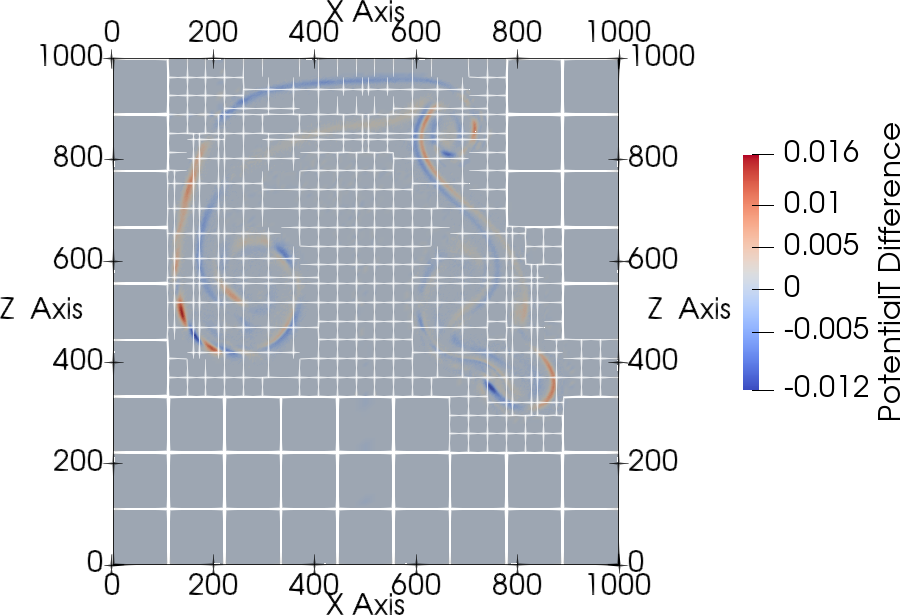
\includegraphics[width=0.55\textwidth]{ppam_two_bubbles_amr_error}
%   }
 \caption*{Potential temperature of fully refined solution minus AMR solution.}
   \end{figure}
\end{frame}

\begin{frame}{3D Cosine Bubble\footfullcite{kelly2012continuous}}
  \begin{columns}
    \begin{column}{0.6\textwidth}
  \begin{center}
    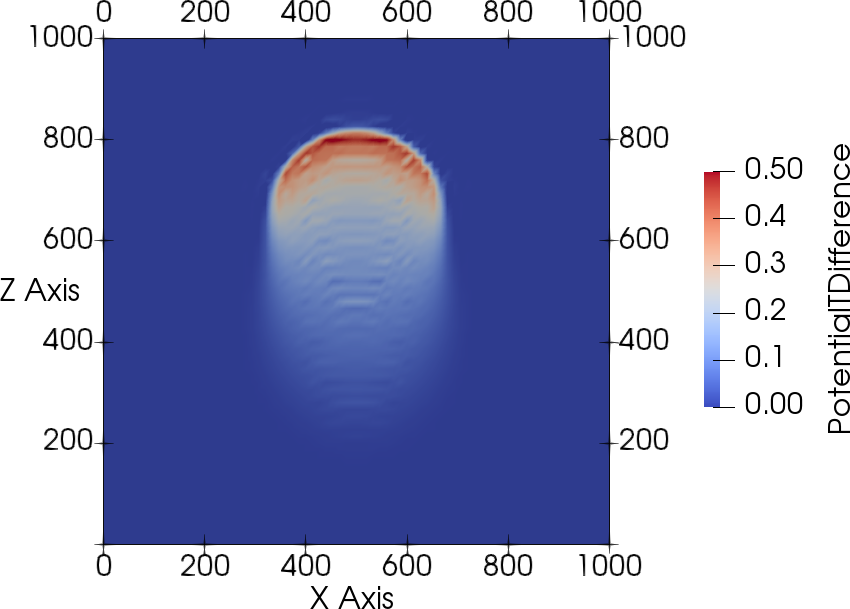
\includegraphics[width=0.85\textwidth]{ppam_cosine_bubble_3d}
  \end{center}
    \end{column}
    \begin{column}{0.4\textwidth}
      \begin{itemize}
      \item Polynomial Order 3
      \item $25^3$ cells
      \item Time: \SI{400}{\s}
      \item Viscosity: $\mu = 0.05$
      \end{itemize}
    \end{column}

  \end{columns}
\end{frame}


\begin{frame}{MUSCL-Hancock Scheme}
  Finite Volume scheme: store only \textbf{cell averages}

  \textbf{Reconstruction} of linear function

  \textbf{Second order} in time and space\footfullcite{vanLeer1979towards}

  \textbf{Stabilized} with (Van Albada~\footfullcite{van1997comparative}) slope limiter

  Very stable, larger \textbf{numerical viscosity}
\end{frame}

\begin{frame}
  \frametitle{Two Bubbles: Finite Volume}
  \begin{columns}
    \begin{column}{0.6\textwidth}
  \begin{center}
    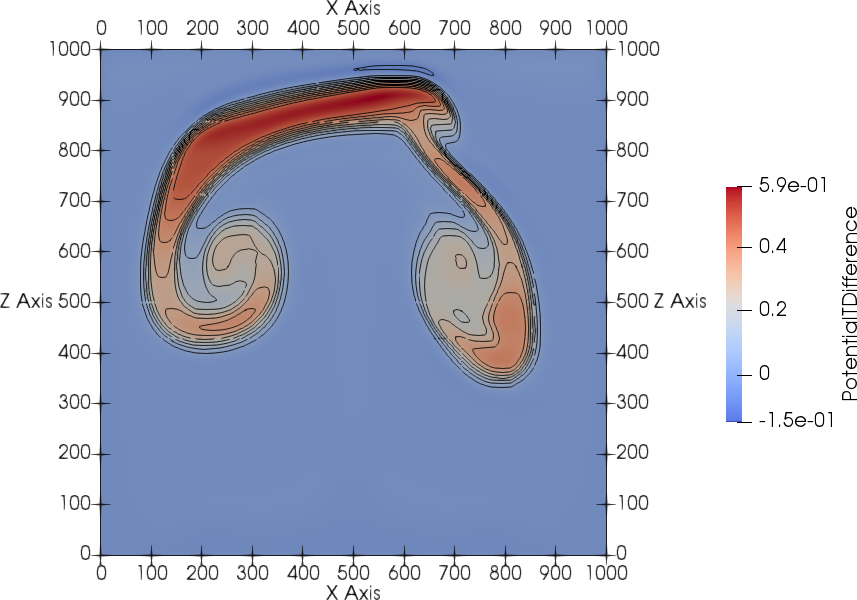
\includegraphics[width=1.0\textwidth]{paper_two_bubbles_fv}
  \end{center}
    \end{column}
    \begin{column}{0.4\textwidth}
      \begin{itemize}
      \item $7^2$ patches with $90^2$ cells each
      \item Euler equations ($\mu = 0$)
      \item Numerical viscosity smooths solution
      \end{itemize}
    \end{column}
  \end{columns}
\end{frame}

\begin{frame}{Summary}
  \begin{block}{Results}
    \begin{itemize}
    \item \textbf{ADER-DG} can be used to simulate Navier-Stokes equations.
    \item Total variation \textbf{measures edges} of numerical solution.
    \item Chebyshev's criterion finds \textbf{interesting cells}.
    \item Combination of both \textbf{accurately tracks} cloud.
    \item AMR solution is close to fully refined solution but needs \textbf{fewer} cells.
    \item \textbf{Artificial viscosity} of finite volume has a similar effect as \textbf{physical viscosity} of Navier-Stokes.  
    \end{itemize}
  \end{block}
\end{frame}

\begin{frame}{Acknowledgments}
This project has received funding from the European Union's Horizon 2020 research and
innovation programme under grant agreement No 823844 (\textbf{ChEESE}) and 671698 (\textbf{ExaHyPE}).

\begin{center}

\includegraphics[width=0.7\textwidth]{logos}
\end{center}
\end{frame}

\begin{frame}
  \frametitle{Shared-Memory Scaling (from\footfullcite{reinarz2019exahype})}

  \begin{center}
  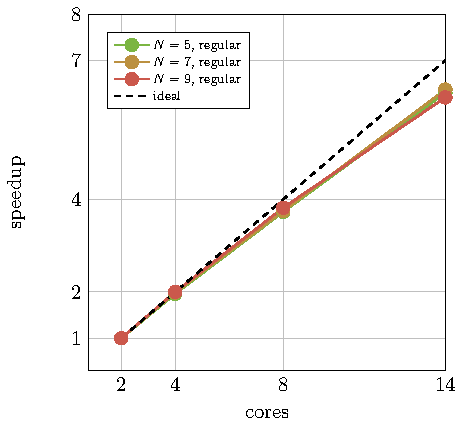
\includegraphics[width=0.4\textwidth]{speedup_tbb}
  \end{center}
  
\end{frame}
\end{document}